\subsection{Structural Interpretation: Projective Thermodynamics}
  \label{subsec:structural-interpretation-projective-thermodynamics}

  This subsection provides a unifying structural interpretation of several results
  developed throughout this work.
  It does not introduce new dynamical assumptions, but makes explicit a mechanism
  that has been implicitly operative in the preceding sections, linking projection,
  bounded relaxation, and effective observables.

  In the Cosmochrony framework, physical observables arise through a projection
  $\Pi : \Omega \rightarrow O$ from the relational configuration space $\Omega$ of the
  $\chi$ substrate.
  As established earlier, this projection is generically non-injective.
  Violations of Bell inequalities demonstrate that distinct underlying configurations
  may be structurally identified at the level of effective observables, even when the
  substratic dynamics remains strictly local.

  The relational substrate $\chi$ relaxes under a bounded flux constraint, naturally
  described by a Born--Infeld-type dynamics.
  This bound limits the admissible transfer of relational relaxation and prevents the
  unbounded accumulation of effective energy, curvature, or other emergent parameters.

  In regimes where the projection remains approximately injective, standard local
  descriptions apply, including classical thermodynamics and smooth geometric
  manifolds.
  However, in saturation regimes---such as strong-field configurations, horizons, or
  magnetically guided dilute plasmas---the projection becomes strongly non-injective.
  The resulting loss of distinguishability induces a structural entropy associated
  with the projection itself,
  \begin{equation}
    S_{\Pi} = -\sum_{o \in O} \mu(\Pi^{-1}(o)) \log \mu(\Pi^{-1}(o)),
  \end{equation}
  which is an objective property of the projection rather than an epistemic measure.

  The structural relations described above may be summarized by a single regime
  diagram, schematically represented in Fig.~\ref{fig:projective-hourglass}.
  This diagram does not depict a causal chain or a dynamical process.
  Rather, it encodes a hierarchy of descriptive validity linking the relational
  substrate, admissibility constraints, projection, and effective observables.
  Each level corresponds to a regime of representation, not to an additional layer
  of physical dynamics.

  \begin{figure}[t]
    \centering
    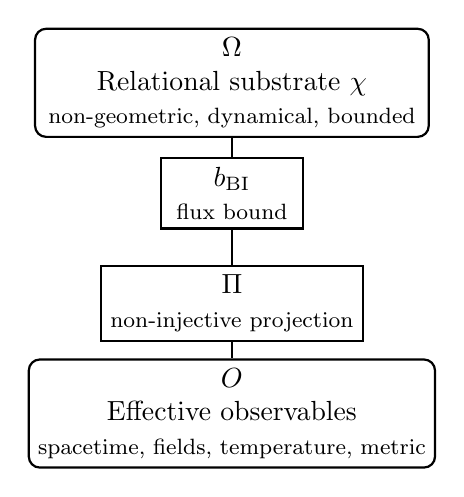
\begin{tikzpicture}[
      node distance=1.4cm,
      every node/.style={align=center},
      box/.style={draw, rounded corners, thick, minimum width=5cm, minimum height=1cm},
      narrow/.style={draw, thick, minimum width=1.8cm, minimum height=0.8cm}
    ]

% Nodes
      \node[box] (omega) {$\Omega$\\Relational substrate $\chi$\\
      {\footnotesize non-geometric, dynamical, bounded}};
      \node[narrow, below of=omega] (bi) {$b_{\mathrm{BI}}$\\
      {\footnotesize flux bound}};
      \node[narrow, below of=bi] (pi) {$\Pi$\\
      {\footnotesize non-injective projection}};
      \node[box, below of=pi] (obs) {$O$\\Effective observables\\
      {\footnotesize spacetime, fields, temperature, metric}};

% Connections
      \draw[thick] (omega) -- (bi);
      \draw[thick] (bi) -- (pi);
      \draw[thick] (pi) -- (obs);

    \end{tikzpicture}
    \caption{Schematic representation of projective regimes in Cosmochrony.
    The relational substrate $\Omega$ undergoes bounded relaxation constrained by
    a Born--Infeld-type flux limit $b_{\mathrm{BI}}$.
    Physical observables arise through a non-injective projection $\Pi$ onto the
    effective space $O$.
    The diagram represents a hierarchy of descriptive regimes rather than a causal
    or dynamical chain.}
    \label{fig:projective-hourglass}
  \end{figure}

  \begin{tcolorbox}[
    colback=gray!5,
    colframe=gray!50,
    boxrule=0.6pt,
    arc=2pt,
    left=6pt,
    right=6pt,
    top=6pt,
    bottom=6pt
  ]
    \textbf{Coronal heating as a projection-limited thermodynamic regime.}

    The coronal heating problem provides a useful illustration of projection-limited
    thermodynamics within the Cosmochrony framework.
    In dense, collisional regimes such as the solar photosphere, the effective mapping
    from underlying relational configurations to fluid observables remains close to
    injective, and standard local thermodynamics applies.

    In contrast, the rarefied and magnetically guided solar corona operates in a regime
    of reduced projectability.
    Many distinct underlying relational configurations are structurally identified by
    the same plasma-level observables.
    In such circumstances, an elevated effective temperature may emerge as a fitting
    parameter absorbing unresolved collective relaxation channels, rather than as a
    direct proxy for local collisional energy density.

    From this viewpoint, nanoflare activity and Alfv\'en-like transport do not represent
    ad hoc heating sources.
    Instead, they reflect the redistribution of relaxation flux under a bounded-transfer
    constraint, consistent with a Born--Infeld-type saturation of admissible effective
    channels.
    The coronal temperature anomaly thus signals a transition between projective
    regimes, rather than a failure of the underlying dynamics.
  \end{tcolorbox}

  The upper part of the diagram represents the infra-physical regime, where the
  $\chi$ substrate evolves through strictly local and bounded relaxation without
  reference to spacetime geometry.
  The central constriction reflects the universal bound on relational flux, which
  limits admissible transfer and prevents divergence of effective observables.
  The projection $\Pi$ selects a reduced set of admissible configurations, inducing
  structural non-injectivity and loss of distinguishability.
  The lower level corresponds to effective physical descriptions, where thermodynamic
  and geometric parameters act as compensatory descriptors of unresolved relational
  structure.

  Within this perspective, effective parameters such as temperature or metric
  curvature emerge as Lagrange multipliers absorbing unresolved relational complexity.
  High effective temperatures or anomalous geometric features therefore do not signal
  excess local energy density or exotic substratic dynamics, but reflect the
  compression of a bounded relational flux into a reduced observable description.

  An analogous interpretation applies to geometric observables.
  Metric curvature, horizon formation, and related spacetime features act as effective
  descriptors compensating for the saturation of admissible relational flux.
  They encode unresolved relational structure within the projected description,
  in direct analogy with thermodynamic variables.
  Such geometric features do not signal a breakdown of the underlying substratic
  dynamics, but rather the progressive loss of validity of local spacetime-based
  descriptions in strongly non-injective projective regimes.

  The bounded character of substratic relaxation plays a decisive role in this
  interpretation.
  It ensures that projection-induced thermodynamic and geometric quantities remain
  finite, rendering the framework predictive and falsifiable despite the
  non-injective nature of the projection.

  This structural mechanism provides a unified interpretation of nonlocal quantum
  correlations, emergent spacetime geometry, and apparent thermodynamic anomalies.
  In all cases, such phenomena reflect the limits of projectability of effective
  descriptions rather than pathologies of the underlying relational dynamics.
